% Options for packages loaded elsewhere
\PassOptionsToPackage{unicode}{hyperref}
\PassOptionsToPackage{hyphens}{url}
%
\documentclass[
]{article}
\title{Exercise\_2}
\author{Diwei\_Zhu}
\date{}

\usepackage{amsmath,amssymb}
\usepackage{lmodern}
\usepackage{iftex}
\ifPDFTeX
  \usepackage[T1]{fontenc}
  \usepackage[utf8]{inputenc}
  \usepackage{textcomp} % provide euro and other symbols
\else % if luatex or xetex
  \usepackage{unicode-math}
  \defaultfontfeatures{Scale=MatchLowercase}
  \defaultfontfeatures[\rmfamily]{Ligatures=TeX,Scale=1}
\fi
% Use upquote if available, for straight quotes in verbatim environments
\IfFileExists{upquote.sty}{\usepackage{upquote}}{}
\IfFileExists{microtype.sty}{% use microtype if available
  \usepackage[]{microtype}
  \UseMicrotypeSet[protrusion]{basicmath} % disable protrusion for tt fonts
}{}
\makeatletter
\@ifundefined{KOMAClassName}{% if non-KOMA class
  \IfFileExists{parskip.sty}{%
    \usepackage{parskip}
  }{% else
    \setlength{\parindent}{0pt}
    \setlength{\parskip}{6pt plus 2pt minus 1pt}}
}{% if KOMA class
  \KOMAoptions{parskip=half}}
\makeatother
\usepackage{xcolor}
\IfFileExists{xurl.sty}{\usepackage{xurl}}{} % add URL line breaks if available
\IfFileExists{bookmark.sty}{\usepackage{bookmark}}{\usepackage{hyperref}}
\hypersetup{
  pdftitle={Exercise\_2},
  pdfauthor={Diwei\_Zhu},
  hidelinks,
  pdfcreator={LaTeX via pandoc}}
\urlstyle{same} % disable monospaced font for URLs
\usepackage[margin=1in]{geometry}
\usepackage{color}
\usepackage{fancyvrb}
\newcommand{\VerbBar}{|}
\newcommand{\VERB}{\Verb[commandchars=\\\{\}]}
\DefineVerbatimEnvironment{Highlighting}{Verbatim}{commandchars=\\\{\}}
% Add ',fontsize=\small' for more characters per line
\usepackage{framed}
\definecolor{shadecolor}{RGB}{248,248,248}
\newenvironment{Shaded}{\begin{snugshade}}{\end{snugshade}}
\newcommand{\AlertTok}[1]{\textcolor[rgb]{0.94,0.16,0.16}{#1}}
\newcommand{\AnnotationTok}[1]{\textcolor[rgb]{0.56,0.35,0.01}{\textbf{\textit{#1}}}}
\newcommand{\AttributeTok}[1]{\textcolor[rgb]{0.77,0.63,0.00}{#1}}
\newcommand{\BaseNTok}[1]{\textcolor[rgb]{0.00,0.00,0.81}{#1}}
\newcommand{\BuiltInTok}[1]{#1}
\newcommand{\CharTok}[1]{\textcolor[rgb]{0.31,0.60,0.02}{#1}}
\newcommand{\CommentTok}[1]{\textcolor[rgb]{0.56,0.35,0.01}{\textit{#1}}}
\newcommand{\CommentVarTok}[1]{\textcolor[rgb]{0.56,0.35,0.01}{\textbf{\textit{#1}}}}
\newcommand{\ConstantTok}[1]{\textcolor[rgb]{0.00,0.00,0.00}{#1}}
\newcommand{\ControlFlowTok}[1]{\textcolor[rgb]{0.13,0.29,0.53}{\textbf{#1}}}
\newcommand{\DataTypeTok}[1]{\textcolor[rgb]{0.13,0.29,0.53}{#1}}
\newcommand{\DecValTok}[1]{\textcolor[rgb]{0.00,0.00,0.81}{#1}}
\newcommand{\DocumentationTok}[1]{\textcolor[rgb]{0.56,0.35,0.01}{\textbf{\textit{#1}}}}
\newcommand{\ErrorTok}[1]{\textcolor[rgb]{0.64,0.00,0.00}{\textbf{#1}}}
\newcommand{\ExtensionTok}[1]{#1}
\newcommand{\FloatTok}[1]{\textcolor[rgb]{0.00,0.00,0.81}{#1}}
\newcommand{\FunctionTok}[1]{\textcolor[rgb]{0.00,0.00,0.00}{#1}}
\newcommand{\ImportTok}[1]{#1}
\newcommand{\InformationTok}[1]{\textcolor[rgb]{0.56,0.35,0.01}{\textbf{\textit{#1}}}}
\newcommand{\KeywordTok}[1]{\textcolor[rgb]{0.13,0.29,0.53}{\textbf{#1}}}
\newcommand{\NormalTok}[1]{#1}
\newcommand{\OperatorTok}[1]{\textcolor[rgb]{0.81,0.36,0.00}{\textbf{#1}}}
\newcommand{\OtherTok}[1]{\textcolor[rgb]{0.56,0.35,0.01}{#1}}
\newcommand{\PreprocessorTok}[1]{\textcolor[rgb]{0.56,0.35,0.01}{\textit{#1}}}
\newcommand{\RegionMarkerTok}[1]{#1}
\newcommand{\SpecialCharTok}[1]{\textcolor[rgb]{0.00,0.00,0.00}{#1}}
\newcommand{\SpecialStringTok}[1]{\textcolor[rgb]{0.31,0.60,0.02}{#1}}
\newcommand{\StringTok}[1]{\textcolor[rgb]{0.31,0.60,0.02}{#1}}
\newcommand{\VariableTok}[1]{\textcolor[rgb]{0.00,0.00,0.00}{#1}}
\newcommand{\VerbatimStringTok}[1]{\textcolor[rgb]{0.31,0.60,0.02}{#1}}
\newcommand{\WarningTok}[1]{\textcolor[rgb]{0.56,0.35,0.01}{\textbf{\textit{#1}}}}
\usepackage{graphicx}
\makeatletter
\def\maxwidth{\ifdim\Gin@nat@width>\linewidth\linewidth\else\Gin@nat@width\fi}
\def\maxheight{\ifdim\Gin@nat@height>\textheight\textheight\else\Gin@nat@height\fi}
\makeatother
% Scale images if necessary, so that they will not overflow the page
% margins by default, and it is still possible to overwrite the defaults
% using explicit options in \includegraphics[width, height, ...]{}
\setkeys{Gin}{width=\maxwidth,height=\maxheight,keepaspectratio}
% Set default figure placement to htbp
\makeatletter
\def\fps@figure{htbp}
\makeatother
\setlength{\emergencystretch}{3em} % prevent overfull lines
\providecommand{\tightlist}{%
  \setlength{\itemsep}{0pt}\setlength{\parskip}{0pt}}
\setcounter{secnumdepth}{-\maxdimen} % remove section numbering
\ifLuaTeX
  \usepackage{selnolig}  % disable illegal ligatures
\fi

\begin{document}
\maketitle

\begin{Shaded}
\begin{Highlighting}[]
\FunctionTok{options}\NormalTok{(}\AttributeTok{tinytex.verbose =} \ConstantTok{TRUE}\NormalTok{)}
\end{Highlighting}
\end{Shaded}

\begin{Shaded}
\begin{Highlighting}[]
\FunctionTok{library}\NormalTok{(readr)}
\FunctionTok{library}\NormalTok{(igraph)}
\end{Highlighting}
\end{Shaded}

\begin{verbatim}
## Warning: package 'igraph' was built under R version 4.1.3
\end{verbatim}

\begin{verbatim}
## 
## Attaching package: 'igraph'
\end{verbatim}

\begin{verbatim}
## The following objects are masked from 'package:stats':
## 
##     decompose, spectrum
\end{verbatim}

\begin{verbatim}
## The following object is masked from 'package:base':
## 
##     union
\end{verbatim}

\begin{Shaded}
\begin{Highlighting}[]
\FunctionTok{library}\NormalTok{(ggraph)}
\end{Highlighting}
\end{Shaded}

\begin{verbatim}
## Warning: package 'ggraph' was built under R version 4.1.3
\end{verbatim}

\begin{verbatim}
## Loading required package: ggplot2
\end{verbatim}

\hypertarget{create-edge-list}{%
\subsection{Create edge list}\label{create-edge-list}}

create the edges data frame and plot a undirected graph.

\begin{Shaded}
\begin{Highlighting}[]
\NormalTok{from\_ }\OtherTok{\textless{}{-}} \FunctionTok{c}\NormalTok{(}\StringTok{"1"}\NormalTok{,}\StringTok{"2"}\NormalTok{,}\StringTok{"3"}\NormalTok{,}\StringTok{"3"}\NormalTok{,}\StringTok{"3"}\NormalTok{,}\StringTok{"3"}\NormalTok{,}\StringTok{"3"}\NormalTok{,}\StringTok{"4"}\NormalTok{,}\StringTok{"5"}\NormalTok{,}\StringTok{"5"}\NormalTok{,}\StringTok{"6"}\NormalTok{,}\StringTok{"6"}\NormalTok{,}\StringTok{"D"}\NormalTok{,}\StringTok{"D"}\NormalTok{,}\StringTok{"B"}\NormalTok{,}\StringTok{"B"}\NormalTok{,}\StringTok{"A"}\NormalTok{)}
\NormalTok{to\_ }\OtherTok{\textless{}{-}} \FunctionTok{c}\NormalTok{(}\StringTok{"2"}\NormalTok{,}\StringTok{"A"}\NormalTok{,}\StringTok{"D"}\NormalTok{,}\StringTok{"C"}\NormalTok{,}\StringTok{"B"}\NormalTok{,}\StringTok{"4"}\NormalTok{,}\StringTok{"5"}\NormalTok{,}\StringTok{"C"}\NormalTok{,}\StringTok{"D"}\NormalTok{,}\StringTok{"6"}\NormalTok{,}\StringTok{"D"}\NormalTok{,}\StringTok{"B"}\NormalTok{,}\StringTok{"B"}\NormalTok{,}\StringTok{"C"}\NormalTok{,}\StringTok{"C"}\NormalTok{,}\StringTok{"A"}\NormalTok{,}\StringTok{"C"}\NormalTok{)}

\NormalTok{egde }\OtherTok{\textless{}{-}} \FunctionTok{data.frame}\NormalTok{(}\AttributeTok{from =}\NormalTok{ from\_, }\AttributeTok{to=}\NormalTok{to\_)}
\NormalTok{g }\OtherTok{\textless{}{-}} \FunctionTok{graph\_from\_data\_frame}\NormalTok{(egde, }\AttributeTok{directed=}\ConstantTok{FALSE}\NormalTok{)}
\NormalTok{g}
\end{Highlighting}
\end{Shaded}

\begin{verbatim}
## IGRAPH 0a2acd4 UN-- 10 17 -- 
## + attr: name (v/c)
## + edges from 0a2acd4 (vertex names):
##  [1] 1--2 2--A 3--D 3--C 3--B 3--4 3--5 4--C 5--D 5--6 6--D 6--B D--B D--C B--C
## [16] B--A A--C
\end{verbatim}

Plot the network with seat label next to each node.

\begin{Shaded}
\begin{Highlighting}[]
\FunctionTok{plot}\NormalTok{(g, }\AttributeTok{layout=}\NormalTok{layout.fruchterman.reingold,}
    \AttributeTok{vertex.size =} \DecValTok{10}\NormalTok{,}
    \AttributeTok{vertex.label =} \FunctionTok{V}\NormalTok{(g)}\SpecialCharTok{$}\NormalTok{name, }\CommentTok{\# Set the labels (Node)}
    \AttributeTok{vertex.label.cex =} \FloatTok{0.8}\NormalTok{,   }\CommentTok{\# Slightly smaller font}
    \AttributeTok{vertex.label.dist =} \FloatTok{1.5}\NormalTok{,  }\CommentTok{\# Offset the labels}
    \AttributeTok{vertex.label.color =} \StringTok{"black"}\NormalTok{,}
    \AttributeTok{vertex.color =} \StringTok{"orange"}\NormalTok{)}
\end{Highlighting}
\end{Shaded}

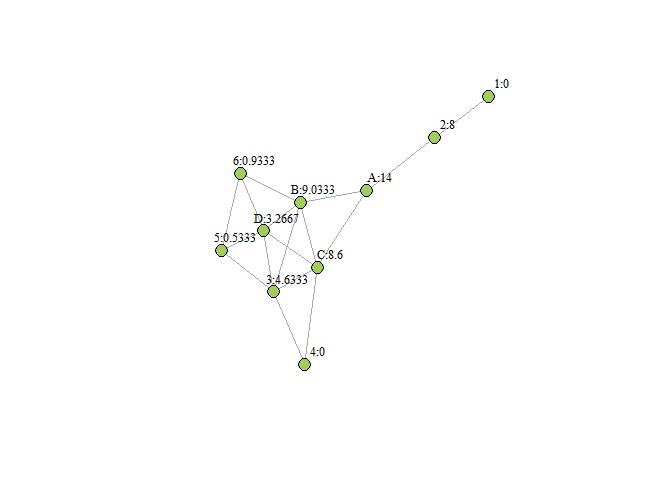
\includegraphics{HW2_files/figure-latex/unnamed-chunk-4-1.pdf}

\hypertarget{betweenness-centrality}{%
\subsection{Betweenness Centrality}\label{betweenness-centrality}}

Calculate betweenness centrality and display the values.

\begin{Shaded}
\begin{Highlighting}[]
\NormalTok{bc }\OtherTok{\textless{}{-}} \FunctionTok{betweenness}\NormalTok{(g)}
\NormalTok{bc}
\end{Highlighting}
\end{Shaded}

\begin{verbatim}
##          1          2          3          4          5          6          D 
##  0.0000000  8.0000000  4.6333333  0.0000000  0.5333333  0.9333333  3.2666667 
##          B          A          C 
##  9.0333333 14.0000000  8.6000000
\end{verbatim}

Plot the network graph with labels and betweenness centrality values.

\begin{Shaded}
\begin{Highlighting}[]
\FunctionTok{V}\NormalTok{(g)}\SpecialCharTok{$}\NormalTok{betweenness }\OtherTok{\textless{}{-}} \FunctionTok{round}\NormalTok{(}\FunctionTok{betweenness}\NormalTok{(g),}\DecValTok{4}\NormalTok{)}
\NormalTok{label1 }\OtherTok{\textless{}{-}} \FunctionTok{paste}\NormalTok{(}\FunctionTok{V}\NormalTok{(g)}\SpecialCharTok{$}\NormalTok{name,}\FunctionTok{V}\NormalTok{(g)}\SpecialCharTok{$}\NormalTok{betweenness,}\AttributeTok{sep=}\StringTok{":"}\NormalTok{)}
  
\FunctionTok{plot}\NormalTok{(g, }\AttributeTok{layout=}\NormalTok{layout.fruchterman.reingold,}
    \AttributeTok{vertex.size =} \DecValTok{10}\NormalTok{,          }
    \AttributeTok{vertex.label =}\NormalTok{ label1, }\CommentTok{\# Set the labels (Node:betweenness)}
    \AttributeTok{vertex.label.cex =} \FloatTok{0.8}\NormalTok{,   }
    \AttributeTok{vertex.label.dist =} \DecValTok{2}\NormalTok{,  }
    \AttributeTok{vertex.label.color =} \StringTok{"black"}\NormalTok{,}
    \AttributeTok{vertex.color =} \StringTok{"darkolivegreen3"}\NormalTok{)}
\end{Highlighting}
\end{Shaded}

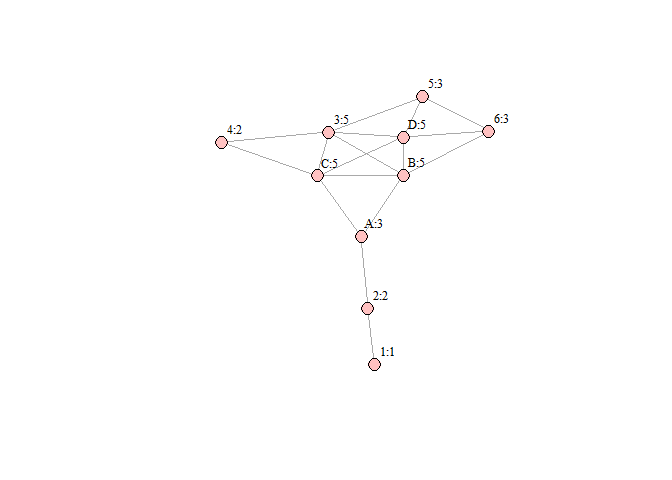
\includegraphics{HW2_files/figure-latex/unnamed-chunk-6-1.pdf}

\hypertarget{degree-centrality}{%
\subsection{Degree Centrality}\label{degree-centrality}}

Calculate degree centrality and display the values.

\begin{Shaded}
\begin{Highlighting}[]
\NormalTok{dc }\OtherTok{\textless{}{-}} \FunctionTok{degree}\NormalTok{(g)}
\NormalTok{dc}
\end{Highlighting}
\end{Shaded}

\begin{verbatim}
## 1 2 3 4 5 6 D B A C 
## 1 2 5 2 3 3 5 5 3 5
\end{verbatim}

Plot the network graph with labels and degree centrality values.

\begin{Shaded}
\begin{Highlighting}[]
\FunctionTok{V}\NormalTok{(g)}\SpecialCharTok{$}\NormalTok{degree }\OtherTok{\textless{}{-}} \FunctionTok{degree}\NormalTok{(g)}
\NormalTok{label2 }\OtherTok{\textless{}{-}} \FunctionTok{paste}\NormalTok{(}\FunctionTok{V}\NormalTok{(g)}\SpecialCharTok{$}\NormalTok{name,}\FunctionTok{V}\NormalTok{(g)}\SpecialCharTok{$}\NormalTok{degree,}\AttributeTok{sep=}\StringTok{":"}\NormalTok{)}
  
\FunctionTok{plot}\NormalTok{(g, }\AttributeTok{layout=}\NormalTok{layout.fruchterman.reingold,}
    \AttributeTok{vertex.size =} \DecValTok{10}\NormalTok{,          }
    \AttributeTok{vertex.label =}\NormalTok{ label2, }\CommentTok{\# Set the labels (Node:degree)}
    \AttributeTok{vertex.label.cex =} \FloatTok{0.8}\NormalTok{,   }
    \AttributeTok{vertex.label.dist =} \DecValTok{2}\NormalTok{,  }
    \AttributeTok{vertex.label.color =} \StringTok{"black"}\NormalTok{,}
    \AttributeTok{vertex.color =} \StringTok{"rosybrown1"}\NormalTok{)}
\end{Highlighting}
\end{Shaded}

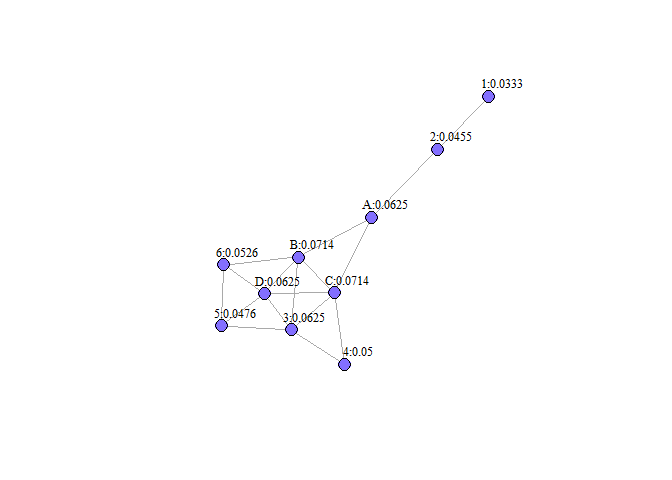
\includegraphics{HW2_files/figure-latex/unnamed-chunk-8-1.pdf}

\hypertarget{closeness-centrality}{%
\subsection{Closeness Centrality}\label{closeness-centrality}}

Calculate closeness centrality and display the values.

\begin{Shaded}
\begin{Highlighting}[]
\NormalTok{cc }\OtherTok{\textless{}{-}} \FunctionTok{closeness}\NormalTok{(g)}
\NormalTok{cc}
\end{Highlighting}
\end{Shaded}

\begin{verbatim}
##          1          2          3          4          5          6          D 
## 0.03333333 0.04545455 0.06250000 0.05000000 0.04761905 0.05263158 0.06250000 
##          B          A          C 
## 0.07142857 0.06250000 0.07142857
\end{verbatim}

Plot the network graph with labels and closeness centrality values.

\begin{Shaded}
\begin{Highlighting}[]
\FunctionTok{V}\NormalTok{(g)}\SpecialCharTok{$}\NormalTok{closeness }\OtherTok{\textless{}{-}} \FunctionTok{round}\NormalTok{(}\FunctionTok{closeness}\NormalTok{(g),}\DecValTok{4}\NormalTok{)}
\NormalTok{label3 }\OtherTok{\textless{}{-}} \FunctionTok{paste}\NormalTok{(}\FunctionTok{V}\NormalTok{(g)}\SpecialCharTok{$}\NormalTok{name,}\FunctionTok{V}\NormalTok{(g)}\SpecialCharTok{$}\NormalTok{closeness,}\AttributeTok{sep=}\StringTok{":"}\NormalTok{)}
  
\FunctionTok{plot}\NormalTok{(g, }\AttributeTok{layout=}\NormalTok{layout.fruchterman.reingold,}
    \AttributeTok{vertex.size =} \DecValTok{10}\NormalTok{,          }
    \AttributeTok{vertex.label =}\NormalTok{ label3, }\CommentTok{\# Set the labels (Node:closeness)}
    \AttributeTok{vertex.label.cex =} \FloatTok{0.8}\NormalTok{,   }
    \AttributeTok{vertex.label.dist =} \DecValTok{2}\NormalTok{,  }
    \AttributeTok{vertex.label.color =} \StringTok{"black"}\NormalTok{,}
    \AttributeTok{vertex.color =} \StringTok{"slateblue1"}\NormalTok{)}
\end{Highlighting}
\end{Shaded}

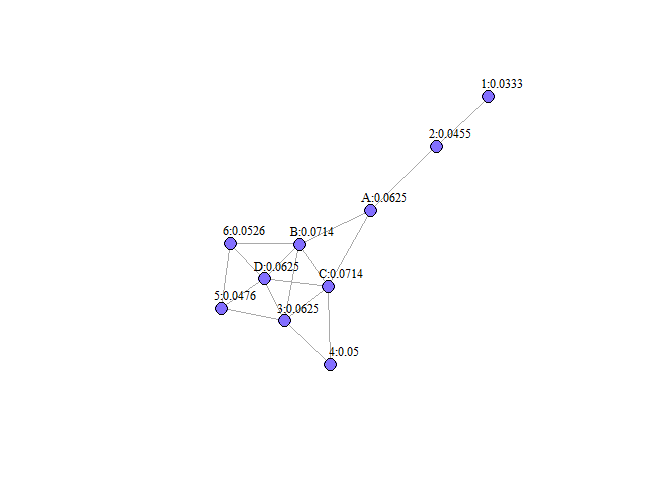
\includegraphics{HW2_files/figure-latex/unnamed-chunk-10-1.pdf}

\hypertarget{choice-of-seat}{%
\subsection{Choice of seat}\label{choice-of-seat}}

We will make decision based on the three measure of centrality we
calculated.

\begin{enumerate}
\def\labelenumi{\arabic{enumi}.}
\tightlist
\item
  Degree Centrality: B, C, and D have degree centrality equal to 5 while
  A has a lower degree centrality at 3. This means that if we sit on B,
  C, or D, there would be more people we can directly talk to.
\item
  Betweenness Centrality: A has an obviously higher betweenness
  centrality at 14, meaning that A is on most of the shortest paths
  between pairs of seats and has a influence on the flow of information
  in the bus. Among B, C, and D, B has the highest betweenness
  centrality value. However, it seems to be rare that the colleagues
  would pass on messages from seat to seat (sounds like what kids would
  do in the classroom).
\item
  Closeness Centrality: The higher the closeness centrality, the shorter
  the sum of shortest paths from a node to other nodes, and the closer
  the node to other nodes. B and C have the same highest closeness
  centrality.
\end{enumerate}

To sum up, I will choose B if the passengers mainly talk to people who
sit next to them, because seat B has the highest degree centrality and
closeness centrality, as well as the second highest betweenness
centrality. However, if passengers on the bus like to pass on messages
from one to another even though the receiver is sitting next to the one
who sent the message, I will choose seat A to capture more information.

\end{document}
